\section{Introduction}


\subsection{Overview}

Edges in real-world networks are often directed, such as links on the world wide web, ``follows'' on Twitter or disease transmission in a social network. When analysing networks, the first quantity that is often considered is the distribution of the degrees of nodes in the network.  In this paper we will consider sampling an i.i.d.\ sequence of in- and out-degrees. Conditional on the total in-degree being equal to the total out-degree, we will then sample a uniform directed graph (digraph) with the given degree sequence. Results on such graphs provide insight into what additional underlying structure a real-world network might have, in comparison with a uniformly random graph with the given degree sequence.

When considering such models, previous work by \citet{cooperSizeLargestStrongly2004} (which we will discuss in more detail in Section \ref{sec.previouswork} below) shows that there exists a phase transition in the strong directed connectivity of the graph. Two vertices are part of the same \emph{strongly connected component} (SCC) if and only if there exists a directed cycle that contains both of them. Above some threshold, there will exist a unique giant SCC that occupies a positive proportion of the vertices whereas, below the threshold no SCC will occupy a positive proportion of the vertices. In this paper we will prove one of the first detailed results about the critical case - specifically, that there exists a sequence of random weighted directed multigraphs that can be understood as the scaling limit of the SCCs when viewed in decreasing order of size.

\subsection{Directed graphs}

\begin{figure}
    \centering
    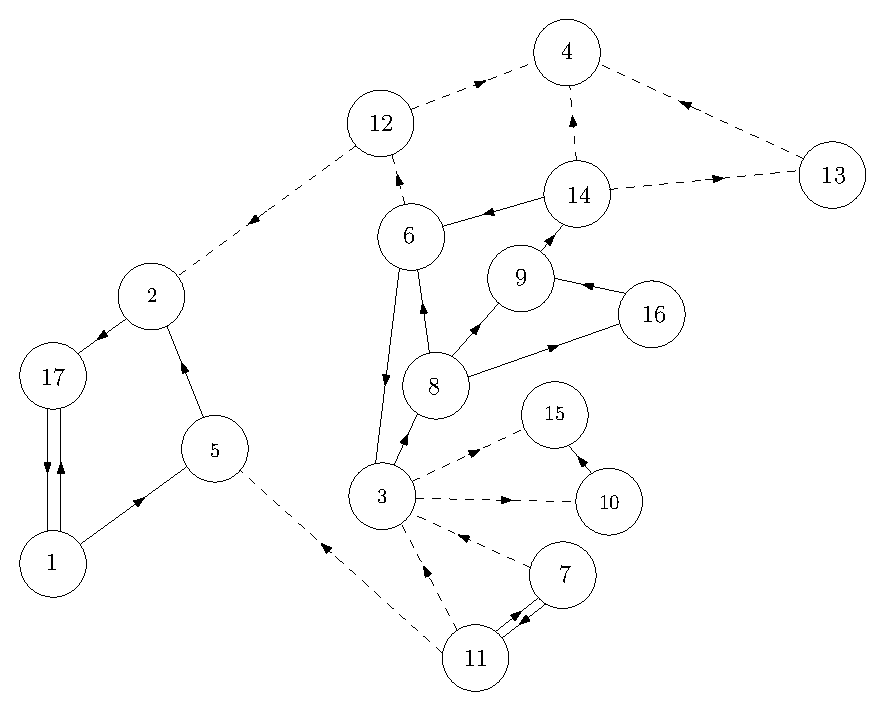
\includegraphics[scale=0.6]{Content/Pictures/biggraph.eps}
    \caption{A directed graph on [17]. The strongly connected components have vertex sets $\{1,2,5,17\}$, $\{3,6,8,9,14,16\}$, $\{7,11\}$, $\{4\}$, $\{10\}$, $\{12\}$, $\{13\}$, and $\{15\}$. Edges that are not part of an SCC are depicted as dashed arrows. Taken from \cite{goldschmidtScalingLimitCritical2019} with permission of the authors.}
    \label{fig.SCCs}
\end{figure}

There are two notions of connectivity when working with a directed graph: weak and strong connectivity. We will be working with the strong notation. We say a vertex $v$ leads to a vertex $w$, written $v \leftarrow w$, if there exists a directed path from $v$ to $w$ in the graph. We say $v$ is \emph{strongly connected} to $w$ if $v$, written $v \leftrightarrow w$ leads to $w$ and $w$ leads to $v$. By convention, $v$ leads to itself. A graph is \emph{strongly connected} if any pair of vertices in the graph are strongly connected. The relation $v \leftrightarrow w$ is an equivalence relation; the digraphs induced by the equivalence classes of $\leftrightarrow$ are referred to as the \emph{strongly connected components} (SCCs). For each vertex $v$ in a directed graph $\vec{G}$, we will use the notation $d^-(v)$ for the in-degree of $v$ and $d^+(v)$ for the out-degree of $v$. Moreover, a directed edge $(v,w)$ has \emph{tail} $v$ and \emph{head} $w$ (see Figure \ref{fig.tailhead}).
\begin{figure}
    \centering
    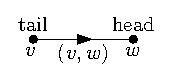
\includegraphics{Content/Pictures/tail_head.eps}
    \caption{An edge $(v,w)$ will be depicted as an arrow from $v$ to $w$.}\label{fig.tailhead}
\end{figure}


\subsection{Description of the model}

First consider a deterministic degree sequence $\vd_1, \ldots, \vd_n$ where $\vd_i = (d_i^-, d_i^+)\in \N \times \N$ for $i = 1, \ldots, n$. We say a directed graph with vertex set $\{1,\dots,n\}$ has degree sequence $\vd_1, \ldots, \vd_n$ if $(d^-(i), d^+(i)) = (d_i^-, d_i^+)$ for $i = 1, \ldots, n$.

In order to sample a uniformly random graph with a given degree sequence, we first consider the \emph{directed configuration model} introduced by \citet{cooperSizeLargestStrongly2004}. Take $n$ vertices $v_1, \ldots, v_n$ such that $v_i$ has $d^-_i$ in-half-edges and $d^+_i$ out-half-edges. Then construct a multigraph by choosing a uniformly random pairing of the in-half-edges with the out-half-edges. \citet{cooperSizeLargestStrongly2004} proved that if we condition on the directed configuration model being simple, we obtain a uniformly chosen random digraph with the given degree sequence.

In this paper we will consider the case where the degree sequence  consists of $n$ i.i.d.\ random variables conditioned on the total in-degree being equal to the total out-degree. So, let $\nu$ be a distribution on $\N \times \N$, and let $\vD_1, \ldots, \vD_n$ be a sequence of i.i.d.\ random variables with distribution $\nu$. We condition on the event
\begin{equation*}
    \left\{ \textstyle \sum_{i=1}^n D_i^- = \sum_{i=1}^n D_i^+ \right\}.
\end{equation*}
Let $\vec{G}_n(\nu)$ be a digraph chosen uniformly at random from all digraphs with degree sequence $\vD_1, \ldots, \vD_n$. We are interested in the limit under rescaling of the SCCs of $\vec{G}_n(\nu)$ as $n\to \infty$.

Suppose $(D^-, D^+) \sim \nu$. We will require the following assumptions to hold:
\begin{enumerate}
    % \item $\E[(D^-) + D^+)^3] < \infty$,
    \item $\E[(D^-)^i(D^+)^j]< \infty$ for $1 \leq i+j\leq 3$, $(i, j) = (1, 3)$ and $(i, j) = (3, 1)$.
    \item $\E[D^-] = \E[D^+]$.
    \item $D^- - D^+$ is strongly aperiodic. This means $D^- - D^+$ is integer-valued and, for all $p > 1$, there does not exist $c \in \R$ such that 
    \begin{equation*}
        \P(D^- - D^+ \in c + p\Z) = 1.
    \end{equation*}
    \item $\E[D^-D^+] = \E[D^{\pm}]$.
\end{enumerate}

The first condition is required to ensure that the steps of a random walk used in the proof have finite variance and thus will convergence (under rescaling) to a Brownian motion. It also ensures similar regularity of other random variables that we use to encode the directed graph. (We discuss relaxing the moment conditions in Subsection \ref{subsec.openproblems}.)

The second and third conditions make sure the event $\{\sum_{i=1}^n D^-_i = \sum_{i=1}^n D^+_i\}$ is well-behaved. The second condition ensures that it is not a large deviation event. Using a result from \citet[Page 42, P1]{spitzerPrinciplesRandomWalk1964}, the third condition ensures that this event has positive probability for all $n \geq 1$. This condition can be relaxed by taking limits for $n \in p \N$ rather than $n \in \N$ where $p$ is the periodicity of $D^- - D^+$. However for simplicity of presentation we will keep it as an assumption.

The fourth assumption is the criticality condition. To understand how this arises, consider the directed configuration model with a deterministic degree sequence $\vd_1, \ldots, \vd_n$ and let $(V, W)$ be a uniformly chosen edge. Since we choose an edge pairing uniformly at random, $W = v_i$ with probability proportional to $d^-_i$. Thus the expected out-degree of $W$ is given by
\begin{align*}
    \E[d^+(W)]
    &= \sum_{i=1}^n d_i^+ \frac{d_i^-}{\sum_{j=1}^n d_j^-}
    = \frac{\sum_{i=1}^n d_i^+ d_i^-}{\sum_{i=1}^n d_j^-}.
\end{align*}
We obtain an identical expression for $\E[d^-(V)]$. Call this quantity $d$. Any other fixed out-edge of $W$ is then distributed approximately like a uniformly chosen edge (here we are ignoring the fact that we have already sampled an edge) and so the out-degree of the head will have mean approximately $d$. Thus if we were to look at the graph of all vertices leading from $W$, it would look approximately like a Bienaymé tree with offspring distribution with mean $d$ \footnote{For $\mu$ a probability distribution on $\N$, a Bienaymé tree with offspring distribution $\mu$ is the family tree of a branching process with offspring distribution $\mu$. Bienaymé trees are often referred to as Galton-Watson trees, but we decide to follow the name change suggested by \citet{addarioberry2021universal}.}. \citet{cooperSizeLargestStrongly2004} show that, under additional assumptions, there exists a phase transition for the existence of a giant SCC depending on whether $d$ is strictly greater than or less than 1. Returning to the random degree sequence and, for now, ignoring conditioning on equal total in- and out-degrees we have
\begin{equation*}
    \frac{\sum_{i=1}^n D_i^+ D_i^-}{\sum_{i=1}^n D_j^{-}}
    \to \frac{\E[D^- D^+]}{\E[D^-]}
\end{equation*}
almost surely as $n \to \infty$ by the law of large numbers. Thus the results of Cooper and Frieze suggest the criticality condition to be $\E[D^- D^+] = \E[D^-]$. Our work in the sequel confirms that this is the case.

We define the following parameters that will determine the behaviour of the SCCs in the limit.
\begin{enumerate}
    \item $\mu:=\E[D^-]=\E[D^+]=\E[D^-D^+]$
    \item $\nu_-:=\frac{\E[(D^-)^2]-\mu}{\mu}$ 
    \item $\sigma_-:=\left(\frac{\mu\E[(D^-)^3]-\E[(D^-)^2]^2}{\mu^2}\right)^{1/2}$ 
    \item $\sigma_+:=\left(\frac{\E[D^-(D^+)^2]-\mu}{\mu}\right)^{1/2}$ 
    \item $\sigma_{-+}:=\frac{\E[(D^-)^2D^+]-\E[(D^-)^2]}{\mu}$ 
\end{enumerate}
% \begin{remark}
% Conditions \ref{cond.beta} and \ref{cond.gamma} ensure that the Central Limit Theorem applies to the fluctuations of the first explored in-degrees around their mean. Condition \ref{cond.critical} ensures that the branching process corresponding to the depth-first exploration (i.e. the exploration of the out-components) is critical. Condition \ref{cond.rho} ensures that this branching process has Brownian scaling. Condition \ref{cond.tau} ensures that the covariance of the in- and out-degrees that are discovered first is finite. Condition \ref{cond.iota} ensures that the strongly connected components are $3$-regular. 
% \end{remark}
\subsection{Metric directed multigraphs and kernels}\label{subsec.mdmkernels}

\begin{figure}[htbp]
    \centering

    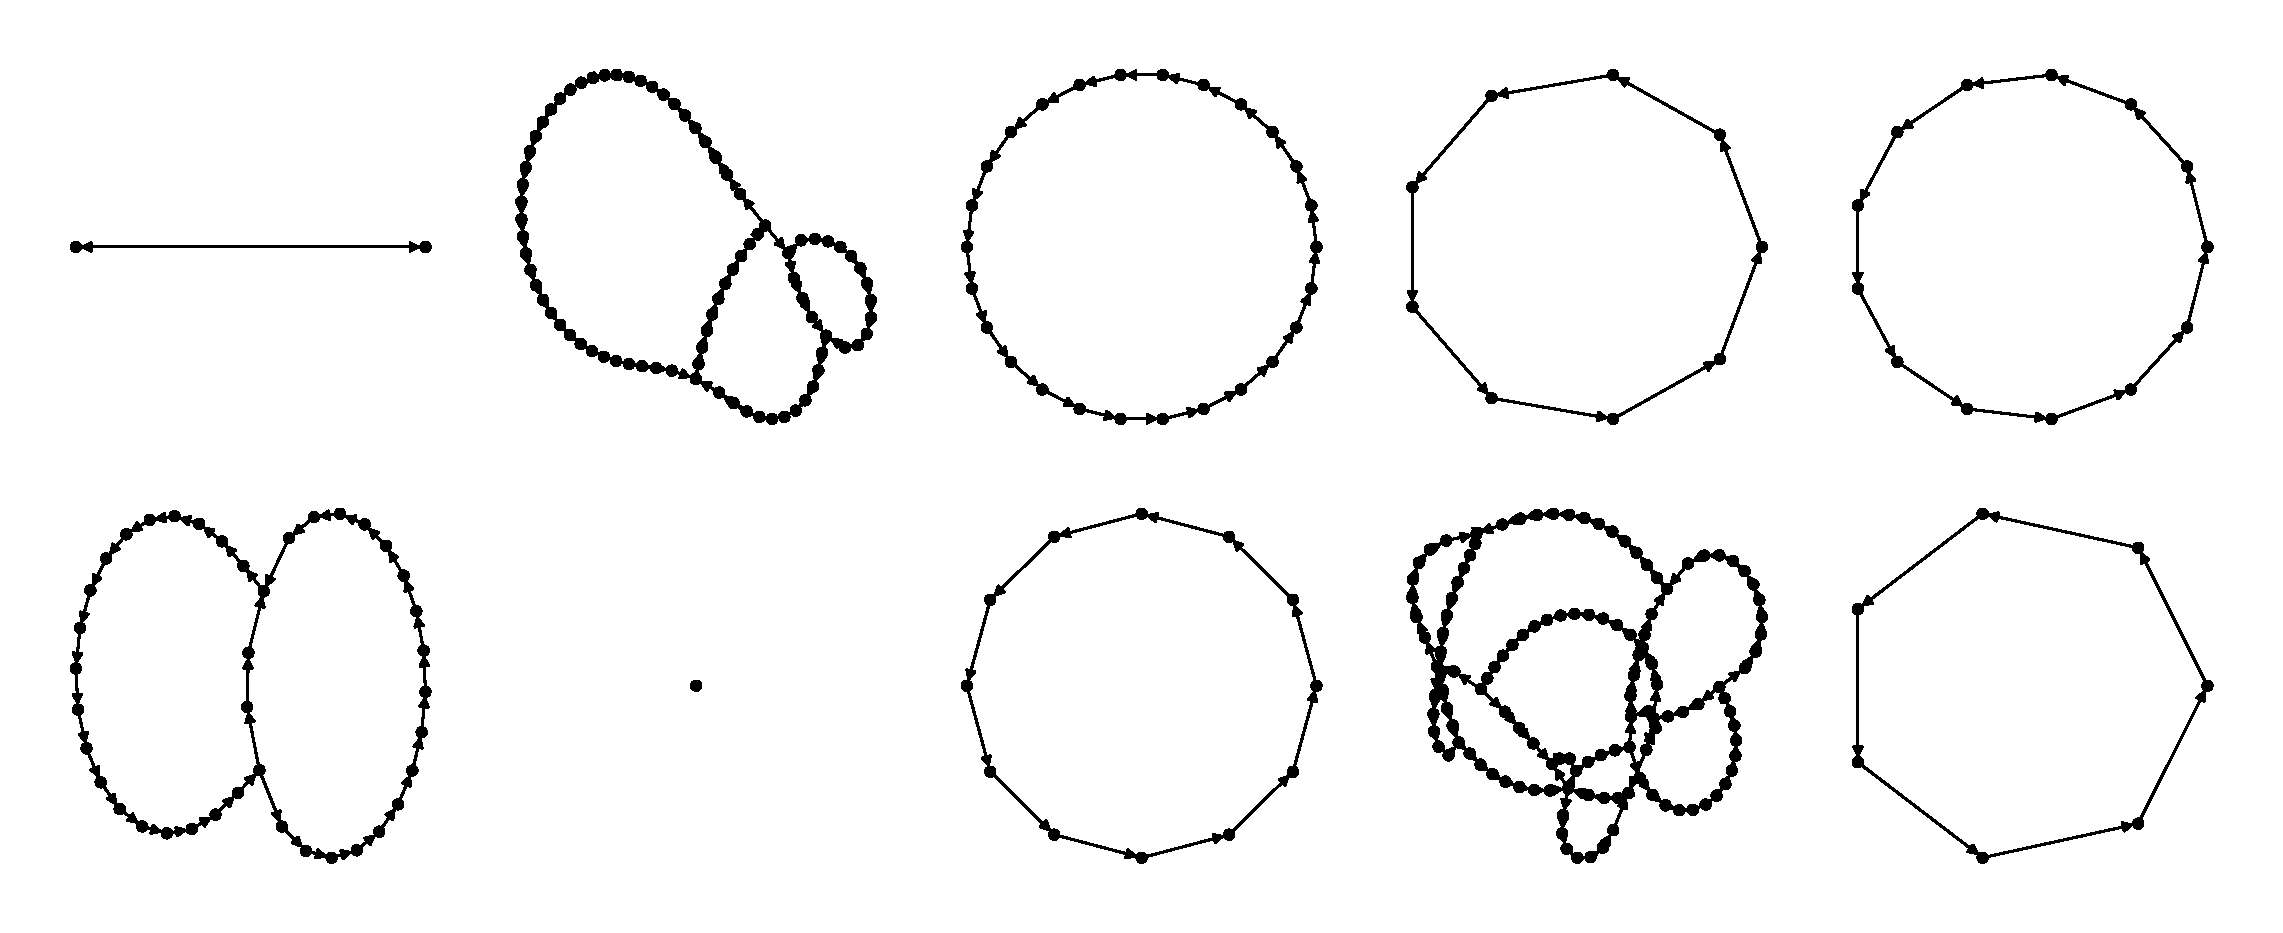
\includegraphics[width=\textwidth]{Content/Pictures/largest_sccs.eps}
    
    \caption{The largest SCC from samples of a directed configuration model with independent $\text{Poisson(1)}$ in- and out-degrees}
    \label{fig:largest-sccs}
\end{figure}

\cref{fig:largest-sccs} shows the largest SCC from samples of a directed configuration model. As can be seen, while the lengths of paths in the SCC are long, the actual structure of the SCC is often quite simple. Previous work by \citet{goldschmidtScalingLimitCritical2019} shows that this is true for the \emph{directed Erdős--Rényi model in the critical window}. The \emph{directed Erd\H{o}s--Rényi model on $n$ vertices with parameter $p$} is a digraph with vertex set $\{1,\dots, n\}$ in which each of the $n(n-1)$ possible directed edges is included with probability $p$ independently. The cases $p=(1+\lambda n^{-1/3})/n$ for $\lambda\in\R$ are referred to as \emph{the critical window}, and the case $p=1/n$ is called \emph{criticality}. In \cite{goldschmidtScalingLimitCritical2019}, it was shown that, for the directed Erdős--Rényi model in the critical window, while the lengths of paths in the SCC scale like $n^{1/3}$, the combinatorial structure of the SCC remains finite. The same turns out to be true in our more general setting.

This idea was formalised in \cite{goldschmidtScalingLimitCritical2019}, and we will use the same formalism in this work. We will first introduce \emph{metric directed multigraphs} (MDMs). These are simply weighted directed multigraphs, but in our context it is more appropriate to think of the weights as lengths, which motivates the change in naming. Formally, a directed multigraph is a tuple $(V, E, r)$ where
\begin{enumerate}
    \item $V$ is a set of vertices,
    \item $E$ is a set of edges, and
    \item $r: E \to V \times V$ is a function mapping each edge to its head and tail; associated with $r$ are two functions $r_1: E \to V$ and $r_2: E \to V$ such that
\begin{equation*}
    r(e) = (r_1(e), r_2(e))
\end{equation*}
for all $e \in E$. $r_1(e)$ is the tail of the edge $e$ and $r_2(e)$ is the head of the edge $e$.
\end{enumerate}
 Then a metric directed multigraph (MDM) is a tuple $M = (V, E, r, l)$ where $(V, E, r)$ is a directed multigraph and $l:E \to [0, \infty)$. Let $\zeroloop$ denote the MDM consisting of a single vertex with a self-loop of length 0.

An \emph{isomorphism} between two MDMs $M = (V, E, r, l)$ and $M' = (V', E', r', l)$ is a pair of functions $(i_V, i_E)$ where $i_V: V \to V'$ and $i_E: E \to E'$ are bijections satisfying the relation
\begin{equation*}
    r'(i_E(e)) = (i_V(r_1(e)), i_V(r_2(e)))
\end{equation*}
for all $e \in E$. We say two MDMs are \emph{isomorphic} if there exists an isomorphism between them. In other words, the MDMs have the same graph structures for their underlying directed multigraphs up to a relabelling of the edges and vertices. Write $\iso(M, M')$ for the set of all isomorphisms between $M$ and $M'$.

We now define a distance $\distmdm$ between two MDMs $M$ and $M'$.  Any isomorphism between $M$ and $M'$ gives a correspondence between the edges of $M$ and the edges of $M'$. We can then take an $\ell_{\infty}$ distance between the lengths of the edges and finally take the isomorphism which minimizes this distance. If $M$ and $M'$ are not isomorphic, we set the distance to be infinite. Formally
\begin{equation*}
    \distmdm(M, M') = \begin{cases}
        \inf_{(i_V, i_E) \in \iso(M, M')} \sup_{e \in E} \abs{l(e) - l(i_E(e))} & \text{if $M$ and $M'$ are isomorphic,} \\
        \infty & \text{otherwise.}
    \end{cases}
\end{equation*}

\begin{figure}[htbp]
    \centering
    \begin{subfigure}[htbp]{0.45\textwidth}
        \centering
        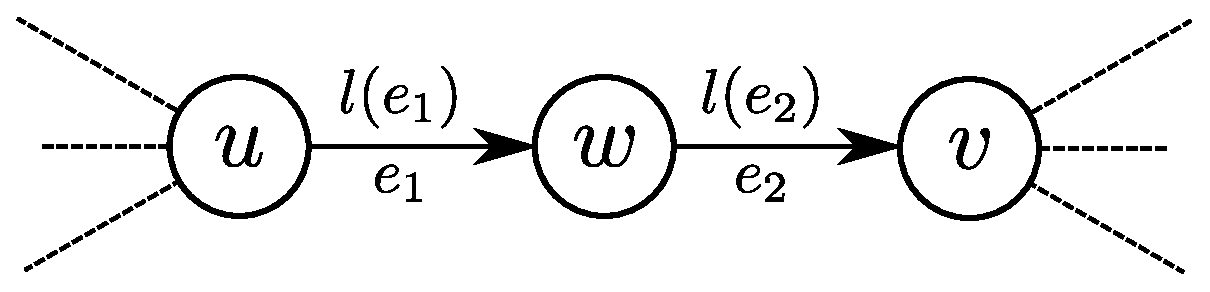
\includegraphics[width=0.95\textwidth]{Content/Pictures/smoothing1.eps}
        \caption{The graph before smoothing $w$}
    \end{subfigure}
    \hfill
    \begin{subfigure}[htbp]{0.45\textwidth}
        \centering
        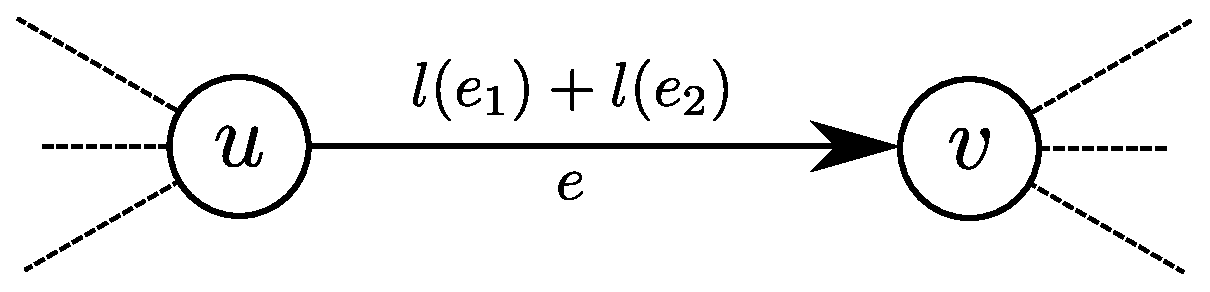
\includegraphics[width=0.95\textwidth]{Content/Pictures/smoothing2.eps}
        \caption{The graph before smoothing $w$}
    \end{subfigure}
    \caption{Smoothing a vertex $w$}
    \label{fig:smoothing}
\end{figure}

\begin{figure}[htbp]
    \centering
    \begin{subfigure}[htbp]{0.45\textwidth}
        \centering
        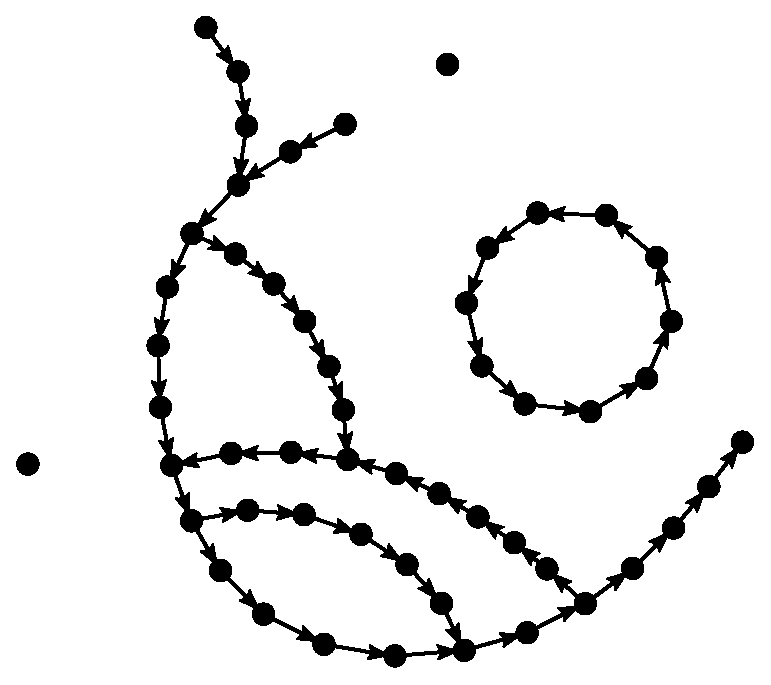
\includegraphics[width=0.90\textwidth]{Content/Pictures/kernel1.eps}
        \caption{$\vec{G}$}
    \end{subfigure}
    \hfill
    \begin{subfigure}[htbp]{0.45\textwidth}
        \centering
        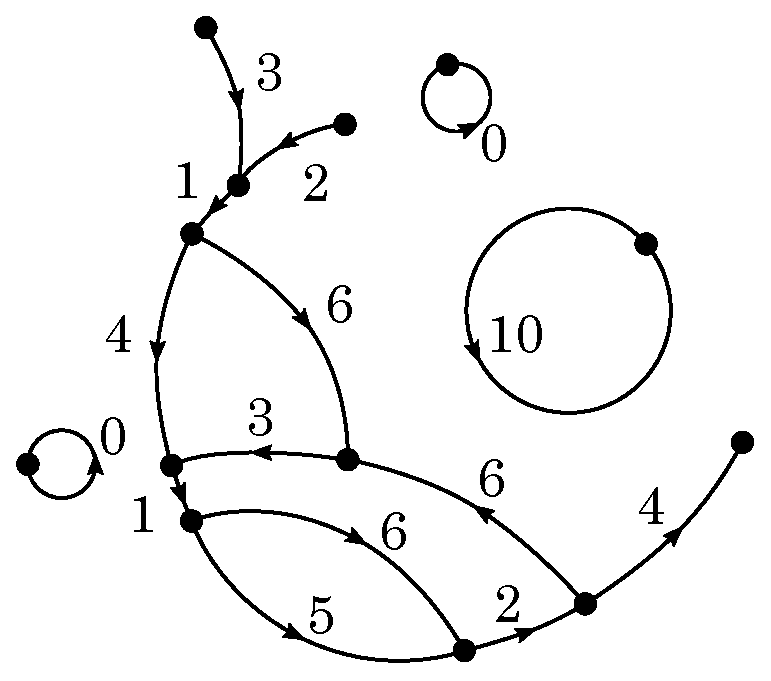
\includegraphics[width=0.90\textwidth]{Content/Pictures/kernel2.eps}
        \caption{$\kernel(\vec{G})$}
    \end{subfigure}
    \caption{An example of a digraph $\vec{G}$ and its kernel $\kernel(\vec{G})$}
    \label{fig:kernel}
\end{figure}

Consider an MDM $M$ and a vertex $w \in M$ with in-degree 1 and out-degree 1 which is not a self-loop. Let $u$ and $v$ be the unique in-neighbour and out-neighbour of $w$ respectively. The MDM obtained by \emph{smoothing} $w$ is obtained by deleting the edges $e_1$ and $e_2$ such that $r(e_1) = (u, w)$ and $r(e_2) = (w, v)$, then adding an edge $e$ such that $r(e) = (u, v)$ and assigning it length $l(e) = l(e_1) + l(e_2)$. This is illustrated in \cref{fig:smoothing}. Then the kernel of a digraph $\vec{G}$ is obtained by doing the following:
\begin{enumerate}
    \item Assign a length $1$ to each edge.
    \item Iteratively smooth vertices with in-degree 1 and out-degree 1 that are not self-loops until there are none remaining.
    \item Replace all singletons by $\zeroloop$.
\end{enumerate}
Denote the resulting MDM by $\kernel(\vec{G})$. An example is shown in \cref{fig:kernel}.

\subsection{Our results}

For $M$ an MDM and $c\in (0,\infty)$, let $cM$ be equal to $M$ with all lengths multiplied by $c$. Let $C_i(n)$ for $i\geq 1$ be the kernels of the SCCs of $\vec{G}_n(\nu)$, listed in decreasing order of size, breaking ties arbitrarily. Complete the list with an infinite repeat of $\zeroloop$. Then, our main theorem is as follows.
\begin{theorem}\label{thm.main}
There exists a sequence $\cC=(\cC_i,i\in \N)$ of random strongly connected MDMs such that, for each $i\geq 1$, $\cC_i$ is either $3$-regular or a loop, and such that 
$$\left(n^{-1/3}C_i(n),i\in \N\right)\todist\left(\cC_i,i\in \N\right)$$
as $n\to \infty$, with respect to the product $d_{\vec{\cG}}$-topology. The law of $\cC=(\cC_i,i\in \N)$ depends only on the parameters $\mu$, $\sigma_+$, and $(\sigma_{-+}+\nu_-)/\mu$.
\end{theorem}
We will describe the limit object and some of its properties in Section \ref{subsec.limitobject}.

We see here why it is important to consider singletons as loops of length zero. For any fixed $k$, the $k$th largest SCC will not be a singleton with high probability. Therefore, no component of our limiting object will be a singleton. Thus we need to pad our SCCs by $\zeroloop$ and consider the kernel of singletons to be $\zeroloop$, to prevent the distance, as defined by $d_{\vec{G}}$, between a singleton in $\left(n^{-1/3}C_i(n),i\in \N\right)$ and any element of $\left(\cC_i,i\in \N\right)$ being infinite.

The law of the limit object places some particular cases of our model in the universality class of the directed Erd\H{o}s--Rényi model as studied by \citet{goldschmidtScalingLimitCritical2019}, although their result holds in a stronger topology. This is the content of the following corollary.
\begin{corollary}\label{cor.erdosrenyi}
Consider $\vec{G}_n(\nu)$, with $\nu$ such that $$\mu=\sigma_+=\sigma_{-+}+\nu_-=1.$$ 
Let $(C_i(n), i\geq 1)$ be the SCCs of $\vec{G}_n(\nu)$. Also consider the directed Erd\H{o}s-R\'enyi model on $n$ vertices at criticality, which we denote by $\vec{G}(n,1/n)$, and let $(C'_i(n), i\geq 1)$ be the SCCs of $\vec{G}_n(\nu)$. Then, $\left(n^{-1/3}C_i(n),i\in \N\right)$ and 
$\left(n^{-1/3}C'_i(n),i\in \N\right)$ have the same limit in distribution in the product $d_{\vec{\cG}}$-topology as $n\to \infty$. 
\end{corollary}
Note that the condition in Corollary \ref{cor.erdosrenyi} is satisfied by $\nu(k^-,k^+)=\nu_1(k^-)\nu_2(k^+)$, with $\nu_i$ the law of a $\operatorname{Poisson}(1)$ random variable.

Moreover, Theorem \ref{thm.main} has the following trivial corollaries, which were previously unknown. 
\begin{corollary}
There exists a random sequence $(\ell_i,i\in \N)\in \R_+^\infty$, such that for $(L^n_i,i\in \N)$ the total lengths in the SCCs of $\vec{G}_n(\nu)$ ordered by decreasing length (appended with an infinite repeat of $0$), and for $(S^n_i,i\in\N)$ the number of vertices in the the SCCs of $\vec{G}_n(\nu)$ ordered by decreasing size (appended with an infinite repeat of $0$),
$$\left(n^{-1/3}L^n_i,n^{-1/3}S^n_i, i\in \N\right)\todist\left(\ell_i,\ell_i,i\in \N\right)$$
as $n\to \infty$ in the product topology on $(\R^2)^\infty$. 
\end{corollary}
\begin{corollary}
For $v,w\in \vec{G}_n(\nu)$ such that $v\to w$, let $d(v,w)$ denote the length of the shortest directed path from $v$ to $w$, and let $$\operatorname{Diam}\left(\vec{G}_n(\nu)\right)=\max_{v,w,\{d(v,w):v\to w\}$$ be the \emph{diameter} of $\vec{G}_n(\nu)$. Then,  $$\operatorname{Diam}\left(\vec{G}_n(\nu)\right)=\Omega(n^{1/3})$$
with high probability.
\end{corollary}


\subsection{Previous work}\label{sec.previouswork}
The configuration model was introduced by \citet{Bollobas1980} to sample a uniformly random graph with a given degree sequence. For a discussion of the configuration model and proofs of standard results, we refer the reader to \cite[Chapter 7]{hofstadRandomGraphsComplex2017}.

Most results on the configuration model are obtained for models with a deterministic degree sequence. The phase transition for the undirected setting was shown in \cite{molloyCriticalPointRandom1995, Molloy1998, Janson2009}. The law of component sizes at criticality and in the critical window were obtained by \citet{Riordan2012} under the assumption that the degrees are bounded. Dhara, van der Hofstad, van Leeuwaarden and Sen showed convergence of the size and surplus edges in the critical window with a finite third moment \cite{Dhara2017} and in the heavy-tailed regime \cite{Dhara2020}.  Bhamidi, Dhara, van der Hofstad and Sen obtained metric space convergence in the critical window in \cite{Bhamidi2020}, a result that the authors later improved to a stronger topology in \cite{Bhamidi2020Glmb}. 

Configuration models with a random degree sequence are considered in \cite{josephComponentSizesCritical2014}, \cite{conchon--kerjanStableGraphMetric2020}, and \cite{Donderwinkel2021heightprocess}. \citet{josephComponentSizesCritical2014} showed convergence of the component sizes and surpluses of the large components under rescaling at criticality, both for degree distributions with finite third moments and for the heavy-tailed regime. \citet{conchon--kerjanStableGraphMetric2020} show Gromov-Hausdorff-Prokhorov convergence at criticality in these two regimes. The results in \cite{conchon--kerjanStableGraphMetric2020} in the heavy-tailed regime are extended to the critical window by D. \cite{Donderwinkel2021heightprocess}. Our techniques are closely related to the techniques introduced in \cite{conchon--kerjanStableGraphMetric2020}. 

Some results have been obtained for other directed graph models. \citet{caoConnectivityGeneralClass2019} consider a class of inhomogeneous directed random graphs. Their results include a phase transition for the existence of a giant SCC. This is a generalisation of work by \citet{Bloznelis2012}, in which a smaller class of inhomogeneous directed graphs is considered. \citet{Samorodnitsky2016} studied the tails of the degree distribution in the directed preferential attachment model. \citet{goldschmidtScalingLimitCritical2019} studied the directed Erd\H{o}s-R\'enyi model, and were the first to obtain metric space convergence of the SCCs of a directed graph. Our methods build on their techniques.

The directed configuration model was first considered by \citet{cooperSizeLargestStrongly2004}. They consider a deterministic degree sequence under a number of conditions. Let $\mu$ be the expected in-egree of a uniformly chosen vertex and $\rho$ be the expected product of the in-degree and out-degree of a uniformly chosen vertex. As discussed previously, a phase transition for the SCCs occurs when $d=\rho/\mu=1$. They show that for $d<1$, with high probability, all SCCs contain $O(\Delta\log(n))$ vertices, for $\Delta$ the maximal degree. On the other hand, for $d>1$, there is a unique SCCs that contains a positive proportion of the vertices and also $O(n)$ edges. Their conditions are restrictive, and include finite second moments of both the in- and out-degree of a uniformly chosen vertex, and a bound of size $n^{1/12}/\log(n)$ on the largest degree. Their proofs are based on an algorithm to explore the directed graph. The condition on the largest degree was later relaxed to $O(n^{1/4})$ by \citet{Graf2016}.

Recently, Cai and Perarnau have obtained a number of results on the directed configuration model with deterministic degrees. In \cite{caiDiameterDirectedConfiguration2020}, they show, under first and second moment conditions of the degree of a uniformly picked vertex, for $d\neq 1$ (i.e. not at criticality), that the diameter of the model on $n$ vertices, rescaled by $\log(n)$ converges to a constant that they identify. Then, in \cite{caiGiantComponentDirected2020}, they show a law of large numbers for the number of vertices and edges in the largest SCC, under slightly stronger moment conditions, and again not at the critical point. In \cite{cai2021rw}, they study the behaviour of a random walk on a directed configuration model.
 
The emergence of a giant weakly connected component for the directed configuration model with a deterministic degree sequence is discussed in the physics literature by \citet{Kryven2016}. He also studies the distribution of the in- and out-components in \cite{Kryven2017}.

The directed configuration model with random in- and out-degrees is also considered by \citet{chenDirectedRandomGraphs2013}, although, importantly, they do not allow for the in- and out-degree of a vertex to be dependent. The authors consider a model in which the in- and out-degrees are two independent sequences of i.i.d.\ random variables drawn from two probability distributions. They propose an algorithm to sample degree sequences that correspond to a simple graph and show the limiting distribution of the degrees generated by this algorithm. 


\subsection{Proof outline}

\def \exploredvertices {\mathcal V}
\def \explorededges {\mathcal E}
\def \forest {F}
\def \edgestack {\mathcal Q}

The techniques we will use to investigate the graph model are a combination of the techniques introduced by Conchon-Kerjan and Goldschmidt in \cite{conchon--kerjanStableGraphMetric2020} and the strategy of Goldschmidt and Stephenson in \cite{goldschmidtScalingLimitCritical2019}. The former work discusses the scaling limit of an undirected uniform graph with i.i.d.\ degrees at criticality, and the latter discusses the scaling limit of the SCCs of a directed Erd\H{o}s-Rényi graph at criticality.

To investigate the structure of the SCCs of a uniformly chosen random graph with degree sequence $(\mathbf{D}_1,\dots,\mathbf{D}_n)$, conditional on $\sum_{i=1}^n D^-_i=\sum_{i=1}^n D^+_i$, we will use an edge-based depth first search procedure (eDFS). This is described in \cref{alg:edfs}. This takes as input a directed multigraph and uses a stack of edges. When the stack is empty, we are at the start of a new out-component and thus pick a new vertex $w$ with probability proportional to its in-degree. Otherwise we remove the last edge $(v, w)$ off the stack. In both cases, if $w$ is not yet in the list of discovered vertices, we add the out-edges from this vertex to the end of the stack of edges (this choice is what makes the exploration depth first) and add $w$ to the list of discovered vertices $\exploredvertices$.  The order in which vertices are added to $\exploredvertices$ is referred to as their order of discovery. Note that we will not discover any vertex with in-degree 0. From the perspective of finding the SCCs, this is not a problem since such vertices will form a singleton SCC.

At each step we also maintain $\hat{s}^-(k)$ and $\hat{s}^+(k)$. $\hat{s}^-(k)$ keeps track of the number of in-edges which we have seen but have not explored the tail of yet at step $k$. $\hat{s}^+(k)$ is akin to a \L{}ukasiewiscz path. At any given step it is equal to the size of the stack of edges after subtracting the number of fully explored out-components.

We also construct a directed forest for which $\hat{s}^+(k)$ will be a true \L{}ukasiewicz path. At each step of the process we will be examining a vertex $w$. If $w$ has not been explored yet then either we are at the start of a new out-component, in which case we add $w$ to the out-forest, or we are exploring an edge $e$ such that $r(e) = (v, w)$ where $v$ has already been explored and added to the out-forest, in which case we add $w$ and the edge $(v, w)$ to the out-forest. If $w$ has already been explored we cannot add $(v, w)$ to the out-forest without creating cycles. Instead add a dummy vertex to the out-forest and an edge from $v$ to the dummy vertex. We call such dummy vertices purple leafs. This is illustrated in Figure \ref{fig.configuration modeloutforest}. We refer to the out-forest corresponding to the exploration up to time $k$ as $\hat{F}_n(k)$.

Consider an edge $e$ in the directed multigraph such that $r(e) = (v, w)$. If $(v, w)$ is not in the out-forest we refer to the edge $e$ as surplus. Such edges will instead correspond to an edge $(v, p)$ in the out-forest where $p$ is a purple leaf.

\begin{algorithm}[htbp]
    \SetAlgoLined
    \KwData{A directed multigraph}
    $\exploredvertices \leftarrow$ an empty ordered list of vertices \tcp*[f]{the list of discovered vertices}\;
    $\edgestack \leftarrow$ an empty ordered list of edges \tcp*[f]{the stack of edges}\;

    $k \leftarrow 0$ \tcp*[f]{the index of the current step} \;
    $\hat{s}^- \leftarrow 0$ \tcp*[f]{the number of seen but unpaired in-edges}\;
    $\hat{s}^+ \leftarrow 0$ \tcp*[f]{the total stack size minus the number of explored out-components} \;
    $\forest \leftarrow$ an empty directed graph \tcp*[f]{the current out-forest}\;
    \While(){there exists undiscovered vertices of positive in-degree}{
        \eIf(\tcp*[f]{we are starting a new out-component}){$\edgestack$ is empty}{
            $w \leftarrow$ a random vertex not in $\exploredvertices$ chosen with prob.\ proportional to $d^-(w)$ \;
            $\hat{s}^+ \leftarrow \hat{s}^+ - 1$ \tcp*[f]{we have finished exploring another out-component} \;
        }(){
            $e \leftarrow$ last edge in $\edgestack$ \;
            remove $e$ from $\edgestack$ \;
            $v \leftarrow$ tail of $e$\;
            $w \leftarrow$ head of $e$ \;
            $\hat{s}^- \leftarrow \hat{s}^- - 1$ \tcp*[f]{we have paired an in-edge} \;
            $\hat{s}^+ \leftarrow \hat{s}^+ - 1$ \tcp*[f]{we have removed and edge from the stack} \;
        }
        \eIf(){$w \not \in \exploredvertices$}{
            append $w$ to $\exploredvertices$ \; 
            add the vertex $w$ to $forest$ \;
            \If(){$\edgestack$ is non-empty}{
                add the edge $(v, w)$ to $\forest$\;
            }
            append all out-edges of $w$ to the end of $\edgestack$ in a uniform random order \;
            $\hat{s}^- \leftarrow \hat{s}^- + d^-(w)$ \tcp*[f]{we've discovered $d^-(w)$ new unpaired in-edges} \;
            $\hat{s}^+ \leftarrow \hat{s}^+ + d^+(w)$ \tcp*[f]{we've added $d^+(w)$ new edges to the stack}\;
        }{
            add a purple leaf to $\forest$ and and edge from $v$ to the leaf \tcp*[f]{we've discovered a surplus edge and add a purple leaf to the forest} \;
        }
        $k \leftarrow k + 1$ \;
        $\hat{s}^-_k \leftarrow \hat{s}^-$ \;
        $\hat{s}^+_k \leftarrow \hat{s}^+$ \;
        $\forest_k \leftarrow \forest$ \;
    }
    \caption{The eDFS procedure \label{alg:edfs}}
\end{algorithm}

\begin{figure}
    \centering
    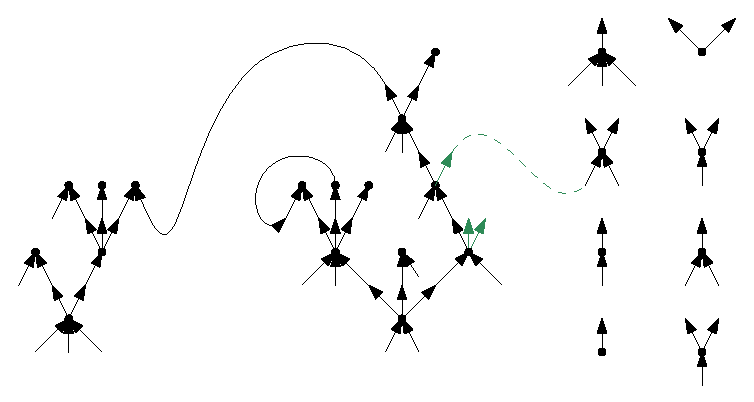
\includegraphics[scale=0.6]{Content/Pictures/configuration_model.eps}
    \caption{The green arrows represent unpaired out-half-edges of vertices that have been visited. One by one, in depth first order, these are paired to a uniform unpaired in-half-edge.}
    \label{fig.configuration model}
\end{figure}

An important motivation for studying the out-forest is the fact that the vertex set of any SCC is contained in one of the components of the out-forest. This is a straightforward property that is further discussed in Lemma \ref{lemma.whatispartofscc}. We have defined the out-forest in such a way that every time step in the exploration corresponds to one vertex in the out-forest. 

A key fact is that the order in which the vertices are discovered does not depend on the position of the purple vertices. Similarly, the position of the purple vertices does not depend on the position of the heads of the surplus edges. Furthermore, we define a necessary condition for a surplus edge to be part of an SCC (see Definition \ref{def.candidate} and Corollary \ref{cor.edgesinSCCs}), and we call surplus edges with this property \emph{candidates}. The candidates are defined in such a way that whether a purple vertex is a candidate does not depend on the position of the heads of the surplus edges. This allows us to define the following sampling procedure. (By slight abuse of notation, we call the purple vertex that corresponds to a surplus edge its tail.)
\begin{enumerate}
    \item We sample the order of discovery of the vertices in the exploration.
    \item We sample at which time steps a surplus edge is added instead of an edge to an undiscovered vertex, which allows us to define the out-forest $(\hat{F}_n(k),k\geq 1)$. 
    \item We visit the purple vertices in $(\hat{F}_n(k),k\geq 1)$ in depth-first order, and for each vertex we sample whether it corresponds to a candidate.
    \item We visit the tails of the candidates in depth-first order, and for each of them, sample where the head of the corresponding surplus edge is.
\end{enumerate}
For an exact description of the sampling procedure, see Subsection \ref{subsec.discrete}. The analogous sampling procedure for the limit object is described in Subsection \ref{subsubsec.samplecontinuousobject}. Then, our approach to show convergence is as follows.

\begin{figure}
    \centering
    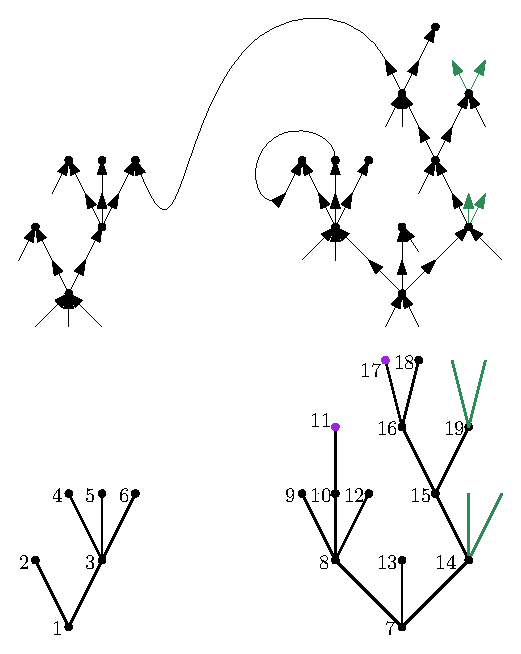
\includegraphics[scale=0.8]{Content/Pictures/configuration_model_out_forest.eps}
    \caption{The out-forest is defined based on the exploration of the digraph. For each surplus edge, we add an extra leaf, which we colour purple. The labels of the vertices correspond to the time step in the exploration at which the vertex is added. The green edges lead to vertices of which the degree and colour have not yet been sampled. We call the depicted forest $\hat{F}_n(19)$.}
    \label{fig.configuration modeloutforest}
\end{figure}

\begin{enumerate}
    \item We find the limit under rescaling of the \L ukasiewicz path and height process of $\hat{F}_n(m_n)$ for $m_n=O(n^{2/3})$ conditional on $\sum_{i=1}^n D^-_i=\sum_{i=1}^n D^+_i$. (For a definition of the \L ukasiewicz path and height process, see \cite{AST_2002__281__R1_0}, Chapter 0.) This is the content of Theorem \ref{thm.convoutforest}. 
    \item We establish that the positions of the tails of the candidates converge. This is the content of Proposition \ref{prop.convergenceancestraledges}, Lemma \ref{prop.extractexcursions}, and Proposition \ref{prop.convergencestartingpointscandidates}.
    \item We show that the positions of the heads of the candidates converge, which is the content of Proposition \ref{prop.convergenceheadscandidates}. 
    \item We identify the tails and heads of the candidates, and recover the SCCs from the resulting digraph with a cutting procedure. We use a result in \cite{goldschmidtScalingLimitCritical2019} that implies that the cutting procedure converges. This summarised in Corollary \ref{cor.sccordereduptotimeT}.
    \item We show that conditioning on the resulting multigraph being simple does not affect the sampling procedure on the time scale $O(n^{2/3})$. This is the content of Proposition \ref{prop.anomalousedges}. 
    \item We prove that for any $\delta>0$, with high probability, all SCCs with length larger than $\delta n^{1/3}$ are contained in the exploration up to time $O(n^{2/3})$. Therefore, we can choose $m_n$ such that, with high probability, we do not miss any large SCCs by not considering the exploration beyond time $m_n$, which finishes the proof of the convergence in the product topology. This is the content of Lemma \ref{lemma.largesccfoundfirst}. 
\end{enumerate}

\subsection{Open problems}\label{subsec.openproblems}
Our work contains the first results on the directed configuration model at criticality, and is the second metric space convergence result for a directed graph model (after the directed Erd\H{o}s-Rényi graph was studied in \cite{goldschmidtScalingLimitCritical2019}), so naturally, there are many interesting unresolved questions.
\begin{enumerate}
    \item The law of our limit object is defined by three parameters that are functions of the (mixed) moments of the degree distribution. Does a different choice of parameters always give a different limit distribution? If so, are the laws absolutely continuous to one another?
    \item Our methods show that the diameter of the configuration model at criticality is  $\Omega(n^{1/3})$, which is in contrast with the off-critical cases (for deterministic degrees), in which the diameter is $O(\log(n))$ \cite{caiDiameterDirectedConfiguration2020}. We believe that the diameter is in fact exactly $O(n^{1/3})$. Goldschmidt and Maazoun are working on this question for the directed Erd\H{o}s-Rényi graph at criticality. 
    \item In \cite{goldschmidtScalingLimitCritical2019}, the authors show convergence of the sequence of SCCs in the $\ell_1$-sense, which is stronger than the product topology as considered by us. This for example implies that for the directed Erd\H{o}s-Rényi graph, under rescaling, the total length in the SCCs converges in distribution to some finite number. Also for undirected configuration models, there are no results that show metric space convergence in a topology on the sequence of components that is stronger than the product topology \cite{Bhamidi2020,conchon--kerjanStableGraphMetric2020,Bhamidi2020Glmb}.
     \item We conjecture that, just like the directed Erd\H{o}s-Rényi graph \cite{goldschmidtScalingLimitCritical2019}, the directed configuration model gives rise to a critical window, that in some sense interpolates between subcritical and supercritical models. It would be interesting to adapt our methods to the critical window.
     \item We plan to extend our understanding of the SCCs by studying the directed graphs that they are embedded in. A first step would be to study all vertices that can be reached from the non-trivial strongly components. This would illuminate connections between the SCCs and expose the fractal structure of the directed graph, which is not observed when only studying the SCCs themselves.
    \item Another natural next step is to study the model under weaker moment conditions. The first condition to eliminate is $\E\left[(D^-)^i(D^+)^j\right]$ for $(i,j)=(1,3)$ and $(i,j)=(3,1)$, which would in some sense makes the identifications less uniform on the ancestral lines. We have reason to believe that this would place the model in  a different universality class, but further research is needed to confirm this. Also the heavy-tailed case is not well-understood, but given our results, it is natural to expect the limit object to be embedded in a tilted stable tree as defined in \cite{conchon--kerjanStableGraphMetric2020}. Moreover, one could define hybrid models by letting the tail-behaviour of the in- and out-degrees be different. 
    \item We conjecture that the inhomogeneous directed random graph model under suitable conditions is part of the same universality class as the directed Erd\H{o}s-Rényi graph \cite{goldschmidtScalingLimitCritical2019} and $\vec{G}_n(\nu)$. We believe that our methods and the methods of \cite{goldschmidtScalingLimitCritical2019} can be adapted to obtain a metric space scaling limit for the inhomogeneous directed random graph model. 

\end{enumerate}

